\clearpage
\section*{September 16, 2026: Dated parcel histories and the parent land rule}
\textit{Agent-drafted research entry.}

A parent's land covariate starts from the tax lots named on its filings,
measured in a reference PLUTO release. That lot often is not the land the
development occupies. Department of Finance (DOF) tax-map histories and dated
maps show how a filing lot relates to the parcels that existed before it, and
correcting the link can change recorded land area by large amounts. The parcel
audit now defines a parent's land as its whole site before the organization
decision, counting each earlier parcel once, and flags a parent when the
available records cannot establish that site. The first complete pass, on
September 15, flagged 166 of 877 weighting parents. The current count is
145 of 905 (116 historical, 29 post-period). A flag records an
unresolved boundary or allocation question, not a proven measurement error.

\subsection*{Why a filing's tax lot can miss the development site}

A BBL (borough, block, lot) identifies a piece of land at a given date. Four
situations separate the filing lot from the development site.

\textit{Mergers into a surviving lot after filing.} DOF often merges a
project's lots after the filing. Sackett's 300-unit filing names lot 47, which
measures 12,500 square feet on the September 2025 map. The March 2026 state
cleanup amendment describes a site containing lots 17 and 47 together, and DOF
merges 47 into 17 in August 2026, after the July 8 sample endpoint.

\textit{Splits.} A development can occupy part of an older lot. At 11 Gerry
Street, production assigned all 111,040 square feet of a predecessor lot; the
mapped filing parcel has 18,044 square feet. Adding every overlapping old lot
can equally pull in another site's land. Proposed splits may be missing from
completed DOF records: Noble/Oak's proposed lot 10 is unmapped.

\textit{Zoning lots with retained buildings or other uses.} A zoning lot can
combine the residential project with land that stays in another use. The
current DOB application for 90 Flatbush Avenue shows a shared zoning site of
lots 1, 7, 10, 13, and 23, covering 61,399 square feet, and NYCIDA's May 12,
2020 board minutes separate a 26,981-square-foot school site from the
residential tower. Suffolk and Norfolk display the same original and zoning
lot lists; their original parcels total 51,879 square feet and the zoning area
is 51,884. Assigning that full area to both parents would count the land twice.

\textit{Lot-number reuse.} The same number can describe different land at
different dates. The Flatbush input at the time was 1,198 square feet, the
area of old lot 23. On February 12, 2020, DOF merger 88954 combined lots 9, 11,
13, 18, 23, and 24 into lot 13, and apportionment 88955 that morning divided the
result into lots 13 and 23. The recreated lot 23 is the 12,603-square-foot
tower parcel (NYCIDA minutes, PDF pages 41 and 49). The 2008 and 2020 dated tax
maps show the change. MapPLUTO 25v4 draws the tower under condominium billing
lot 7502. The candidate land measures differ by a factor of fifty:

\begin{center}
\small
\begin{tabular}{lrl}
\hline
Flatbush land definition & Sq.\ ft. & Evidence \\
\hline
Old lot 23 alone (then in production) & 1,198 & MapPLUTO 18v2\_1 \\
Old lots 18, 23, 24 & 16,531 & DOB original-lot list; 12,240 + 1,198 + 3,093 \\
Recreated tower lot 23 & 12,603 & NYCIDA May 2020 minutes \\
Shared zoning site & 61,399 & Current DOB application \\
\hline
\end{tabular}
\end{center}

The spatial intersection independently finds old lots 18, 23, and 24, matching
the original lot list displayed for DOB job 321595145. Their mapped union is
about 17,980 square feet and the later tower polygon about 12,802; recorded and
polygon areas are separate measurements. The current DOB fields may include
amendments, and the original zoning drawing was not retrievable. The September
21 entry records the production choice of 12,603 square feet and Jacob's
approved estimate of earlier floor area. Smaller cases follow the same pattern:
at 1166 Fox Street, production kept an earlier 2,500-square-foot parcel,
while DOF documents a merger and reapportionment leaving a 10,015-square-foot
filing parcel; Weirfield reuses a lot number after a boundary change, 3,050
square feet in production versus 19,341 in PLUTO 25v4.

\subsection*{The DOF tax-map history snapshot}

DOF publishes transaction-level tax-map records through a public service that
needs no login or key. The project froze a citywide snapshot on September 15,
2026. It has nine tables with 1,589,845 rows:

\begin{center}
\small
\begin{tabular}{lr}
\hline
DOF table & Rows \\
\hline
Current tax-lot polygon attributes, without geometry & 858,065 \\
Current condominium base and billing lots & 12,236 \\
Current condominium unit-to-base links & 307,762 \\
Dated block-map index with PDF links & 93,570 \\
Transaction headers & 78,189 \\
Tax-lot actions & 78,108 \\
Condominium actions & 10,168 \\
Condominium unit actions & 144,198 \\
Tax Map Unit application tracker & 7,549 \\
\hline
\end{tabular}
\end{center}

The headers describe 39,777 distinct transactions from May 20, 2008 to
September 14, 2026. The nine original ZIPs preserve 484 API responses with
exact query URLs and SHA-256 hashes. The service changes over time, so the
snapshot must accompany the replication package.

A transaction lists the lots it retains, drops, and creates. It does not
allocate parts of each old parcel to each new one, and it contains no
historical polygons. An ``Affected'' label means that a lot took part in a map
edit, not that it belongs to the development. DOF transaction dates, tracker
dates, PLUTO dates, filing dates, and developer decision dates are distinct.
The audit walks completed changes backward from each filing lot by date and
time. Where one transaction covers the site completely, this recovers the
earlier parcel set without a spatial threshold. Wyckoff's May 7, 2025
transaction retains lot 19, drops 42 and 51, and creates 20, 21, and 57, giving
old lots 19/42/51 and 50,692 square feet. Third Avenue's December 18, 2025
transaction retains 27, 31, and 35 and drops 30 and 135, a 108-square-foot
frontage strip; the five old lots total 22,247 square feet, against 19,555 in
production. Dated map comparisons then check land coverage and expose sites
that cover only part of a transaction.

\subsection*{The land definition}

The model's land input is the whole parent site before the organization
decision, that is, before the developer chooses between one filing and several
constituent filings. Each earlier parcel counts once, at its recorded tax-lot
area in the reference release: filing-specific PLUTO vintages for historical
parents and PLUTO 23v3\_1 for post-period parents. The September 15 area
review set this as the target measure. Later child lots, cleanup boundaries,
water area, and zoning rights cannot silently substitute for it.

The current rule wording adds the following. For a partial parcel, recorded
legal boundaries or agency plans assign the ground, and a later administrative
successor area can measure that same boundary. Polygons check boundaries; they
do not replace recorded areas. Ground leases contribute their assigned ground.
Separate development rights, nonexclusive easements, retained schools, and
later phases do not automatically add land. Later records can reconstruct the
development ground without establishing ownership at initial filing or the
legal wage-assessment unit. Earlier building floor needs its own allocation,
and later vacancy does not establish earlier vacancy.

\subsection*{The boundary pass rule}

A parent passes when its complete filing ground corresponds to whole earlier
parcels or a documented allocation, with no independent source, filing, or
membership conflict. Three routes establish the boundary.

\textit{Whole earlier parcels by map comparison.} The later filing parcels and
the earlier parcels they overlap must align, with at most 2\% of either union
outside the other. The continuous differences are retained. On September 16,
tightening the tolerance to 1\% or 0.5\% raised the unresolved count from 160
to 165.

\textit{A complete DOF successor set.} The parent contains every successor lot
of a completed DOF transaction, and reversing the transaction recovers exactly
the earlier lot set on the reference map. On September 16 this route passed the
Boyland and Beach 28 Street pairs, at 20,000 and 52,380 square feet, despite
missing later MapPLUTO polygons. A partial successor set cannot pass.

\textit{A documented boundary.} A reviewed recorded boundary, agency plan, or
original filing document supplies the allocation or confirms the whole parcels.

The conflict checks search saved New Building jobs from the Housing Database
and DOB NOW (32,015 on September 16), including small, nonresidential, and
older filings, for other live projects on the same earlier parcels. A DOF
transaction widens that search but does not assign its whole land to a parent.
A filing point locates a record; it does not draw a building footprint. The
Housing Database is not a complete inventory of legacy nonresidential filings.

A flag therefore marks a question to resolve, not a confirmed error or an
automatic request for manual research. Passing means that the available records
support the site under this convention; it does not certify ownership at
filing, complete legal coverage, or a wage-assessment unit. A passing parent
can still carry a candidate area far from production, for example 567 Fulton
Street (279 to 27,542 square feet), 2508 Foster Avenue (1,360 to 11,680), and
643 Degraw Street (1,043 to 9,169) on September 16. Candidate areas stay in the
audit; production land changes only through reviewed decisions in
\path{tasks/parent_opportunities_manual}.

\subsection*{Flag counts}

The September 15 pass flagged 166 of the 877 parents then used for weighting:
120 of 561 historical and 46 of 316 post-period parents. Most of those flags
concerned a site covering only part of a lot-change transaction. Documentary
reviews and parent mergers have since resolved or changed many flags, and the
September 22 source correction, which moved historical proposals to the
inactive-inclusive Housing Database 23Q4 archive, changed the sample itself.
The weighting sample is now 905 parents, of which 145
(116 historical, 29 post-period) are flagged. The two counts use different
samples, so their difference is not a count of resolved cases.

\subsection*{The condominium billing-lot lookup}

The first map comparison replaced condominium billing lots with their physical
base lots and searched the later map only for those base lots. MapPLUTO often
draws condominium land under a billing lot instead, as with Flatbush's lot
7502, so the lookup missed polygons that existed. The corrected lookup uses the
filing BBL when it is mapped, then a physical base lot, then a unique mapped
condominium alias for that base. In the September 16 comparison of the original
166 flagged parents, the fix recovered later footprints for all 19 historical
parents in the missing-map group: four became whole-parcel matches and fifteen
partial-parcel comparisons. The remaining missing-map cases were all
post-period parents.

\begin{figure}[p]
\centering
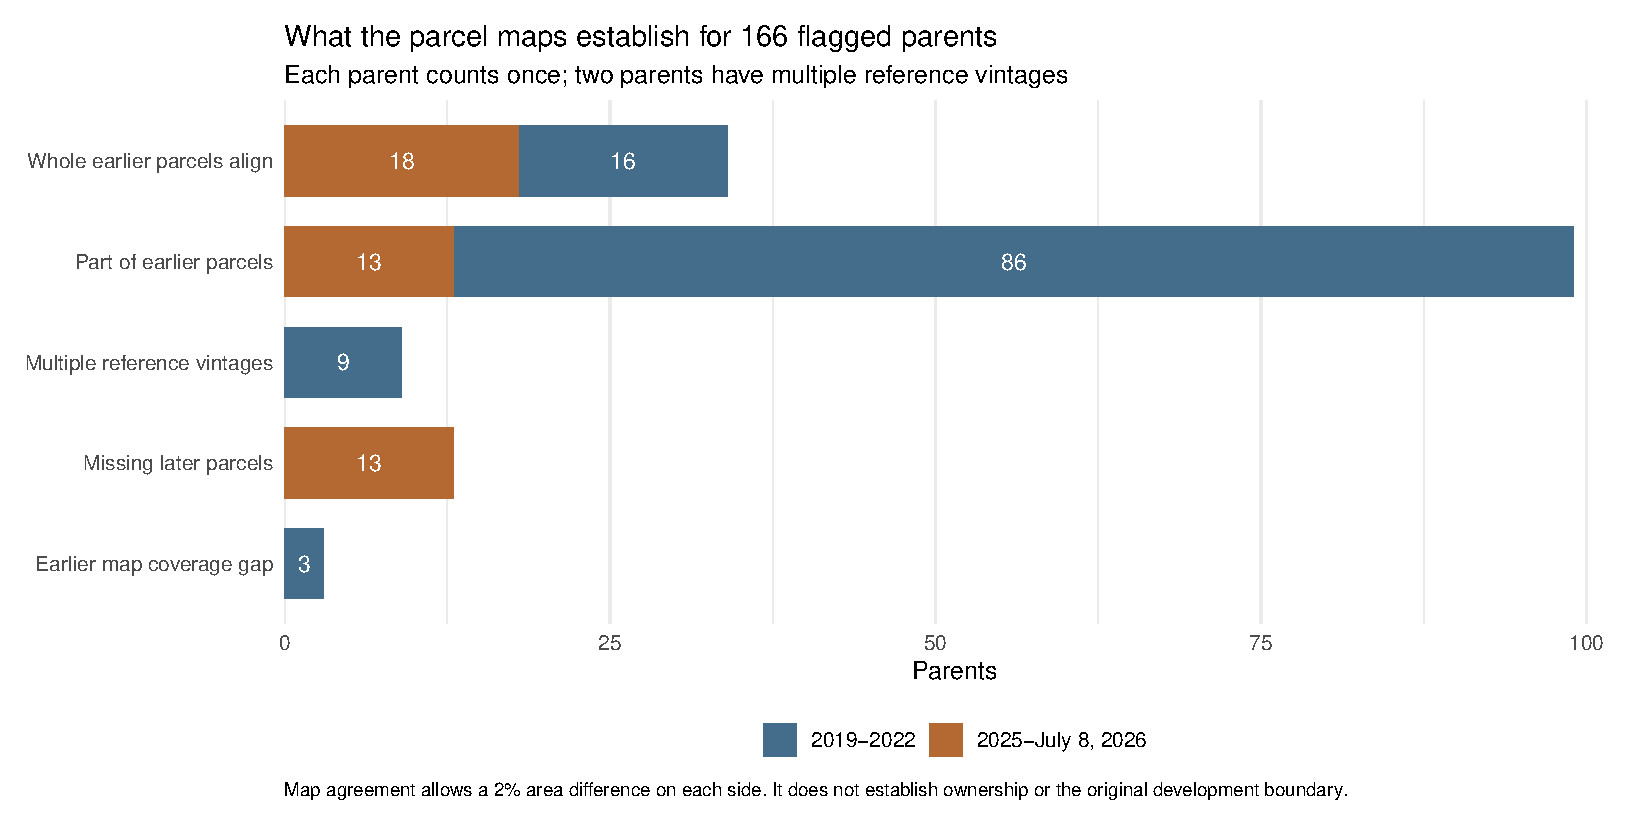
\includegraphics[width=\textwidth,height=.9\textheight,keepaspectratio]{archive/2026-09-16-dof-geometry/dof_geometry_overview.pdf}
\caption{Parcel-map comparison of flagged parents. This is the September 22
version, covering the 158 parents flagged at that time.}
\end{figure}

\subsection*{Magnitudes in a fixed-seed twelve-parent draw}

Before any review, twelve of the 166 flagged parents were drawn with seed
20260915 after sorting by ID: nine historical and three post-period. Two,
Sackett and Noble/Oak, had no settled footprint, leaving ten comparisons of
production area against the summed PLUTO 25v4 lot areas of the mapped filing
parcels. Mean area fell from 50,076.6 to 32,755.5 square feet, a reduction of
17,321.1 square feet, or 34.6\% of the original mean. Seven areas fell and
three rose. The median absolute percentage difference was 55.4\%, and the
median signed change $-26.4\%$. Averaging each parent's percentage change
instead gives $+53.6\%$, because two projects start from very small recorded
areas. Across the ten, PLUTO and the September 15 DOF geometry agree on more
than 99.99\% of their union. On September 21, Godwin's accepted companion lot
88 was added to its parent, so current outputs compare the same IDs against an
updated parent definition. The draw is small, stratified, and conditional on a
flag. It shows that flagged records can hide large measurement problems; it is
not a correction factor for all flagged parents.

\subsection*{Area checks against assessment records}

All ten comparison areas match DOF's final fiscal 2026/27 assessment roll,
and printed map dimensions reproduce seven of them within 0.1\%. Purdy,
Weirfield, and Lorimer lack an independent survey calculation. DOF and PLUTO
share geography and area sources, so their agreement alone does not validate
the measurements. The assessment history also shows update lags: Chatterton
keeps 60,979 square feet in fiscal 2026 and changes to 21,133 in fiscal 2027;
Fox changes from 2,500 to 10,015 between fiscal 2023 and 2024. A matching BBL
must be paired with the boundary in force at the right date.

\textit{Sackett.} The deed in the March 2026 state amendment describes later
lot 17 as a $265\times100$ rectangle, less a $10\times10$ notch, plus a
$10\times100$ access strip: 27,400 square feet. Lot 47 is $125\times100 =
12,500$, together 39,900. The removed neighboring lot 16 measures 8,600 square
feet on the DOF map, although the fiscal 2027 assessment records 12,500; the
map figure conserves the predecessor's 48,500 square feet, whereas summing the
three assessment entries would add 3,900 incorrectly. DOB job B00665570-I1
reports a 48,500-square-foot zoning lot and 300 units, and the August 2025
zoning declaration (CRFN 2025000213962) includes tentative lots 16, 17, and 47.
The 39,900-square-foot sale and cleanup boundary therefore need not equal the
zoning site. Moving from the then production area of 38,500 to 48,500 would
add 10,000 square feet (26.0\%), but the footprint at the February 2022
decision still needs the dated site plan. The live DOB record is not a 2022
snapshot, and the 300 units are an administrative observation, not proof of an
unchanged proposal.

\textit{Noble/Oak.} A city notice for the June 9, 2026 Brooklyn CB1 meeting
describes dividing lot 1 into lots 1 and 10 for two proposed buildings on a
173,834-square-foot site. The full DOF tax-lot polygon measures about 297,134
square feet, near its 299,214-square-foot assessment, while MapPLUTO's
shoreline-clipped polygon measures about 172,691. The difference is mostly a
land definition: the full tax lot includes water, and the onshore site is the
candidate for development land. The earlier clipped polygon measures about
126,049. The 2001 deed runs the boundaries to the centers of Noble, West, and
Oak Streets, and the 2024 deed conveys the same premises with those street
rights, so the map expansion is not itself evidence of land acquired after the
policy. The September 22 entry records the production treatment: the city's
173,834 square feet, which an independent deed reconstruction reproduces as
173,827.90.

\textit{Reproduction note.} Run root \texttt{make site-boundaries}, which
prepares the main data and the DOF snapshot and then runs
\path{tasks/audits/audit_parent_site_boundaries/}. The snapshot is
\path{data_raw/dof_tax_map/2026-09-15/}, owned by
\path{tasks/fetch_dof_tax_map_history/}, whose \path{code/checksums.sha256}
records the frozen bytes. The audit's \path{output/parent_site_scope.csv}
records each weighting parent's flags, evidence, and candidate area, and the
audit's README states the rule. The audit does not
change production land characteristics. The figure is an archived byte copy
whose plotting script was removed after September 22; tag
\texttt{pre-cleanup-2026-09-22} preserves it.
